\documentclass[11pt]{article}
\usepackage[margin=1in]{geometry}
\usepackage{amsmath}
\usepackage{amssymb}
\usepackage[utf8]{inputenc} 
\usepackage{graphicx} 
\usepackage{parskip} 
\usepackage{multirow} 
\usepackage{mathtools}

\DeclarePairedDelimiter\abs{\lvert}{\rvert}%
\DeclarePairedDelimiter\norm{\lVert}{\rVert}%

\makeatletter
\let\oldabs\abs
\def\abs{\@ifstar{\oldabs}{\oldabs*}}

\let\oldnorm\norm
\def\norm{\@ifstar{\oldnorm}{\oldnorm*}}
\makeatother
\usepackage{multicol} 
\usepackage[spanish,es-nodecimaldot]{babel} 
\usepackage{mathtools}
\usepackage{amsfonts}
\usepackage{float}
\usepackage{textcomp}
\usepackage{caption}
\usepackage{subfig}
\usepackage[spanish]{babel}
\usepackage{gensymb}
\def\sen{\mathop{\mbox{\normalfont sen}}\nolimits}

\usepackage{fancyhdr}
\fancyhf{}
\rfoot{\thepage}
\pagestyle{fancy}
\lhead{Nieto Castellanos Fabián}
\chead{}
\rhead{Tarea 9. Histogramas}
\begin{document}

\textbf{1)}
\begin{figure}[H]
\centering
\subfloat[Resolución en el eje $X$ para todos los eventos.]{
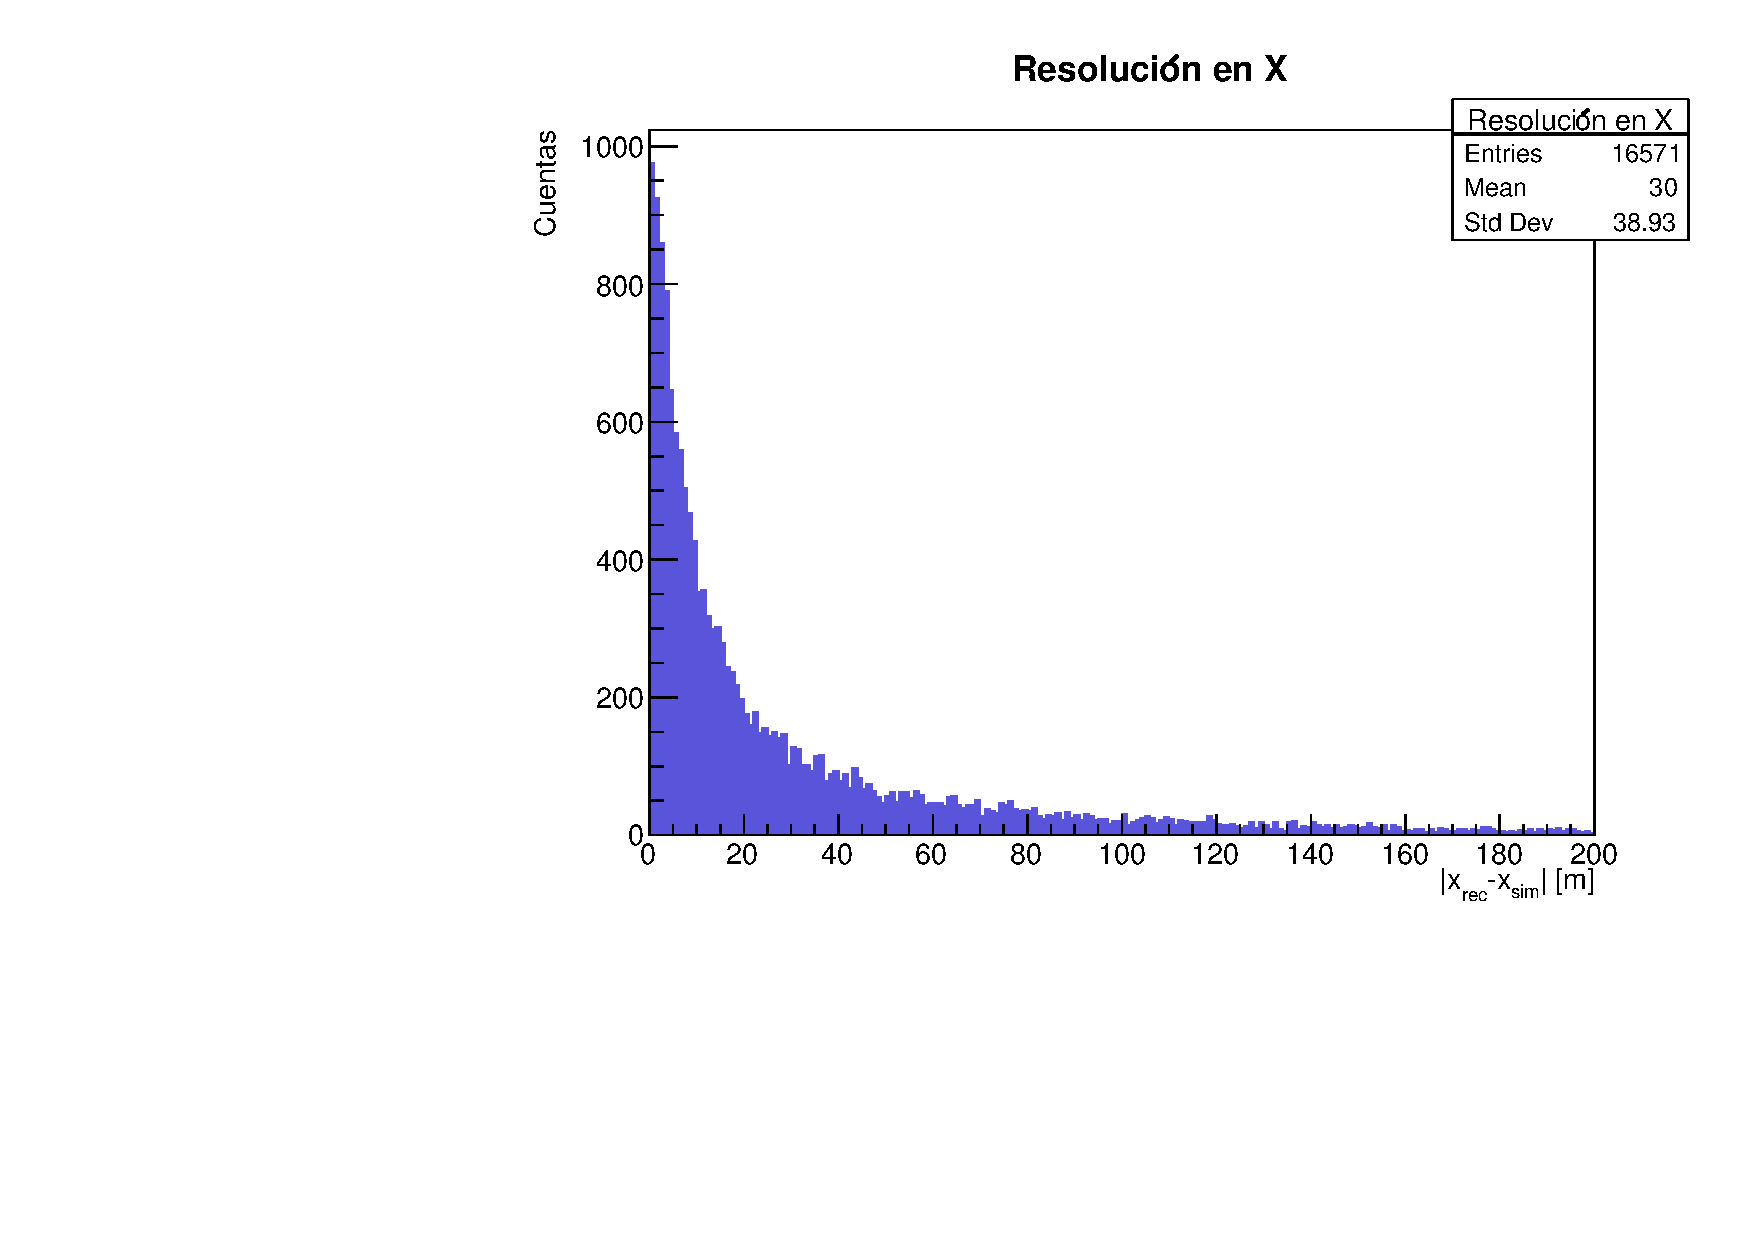
\includegraphics[width=0.8\textwidth]{../Figuras/Prob1A.pdf}}

\subfloat[Resolución en el eje $Y$ para todos los eventos.]{
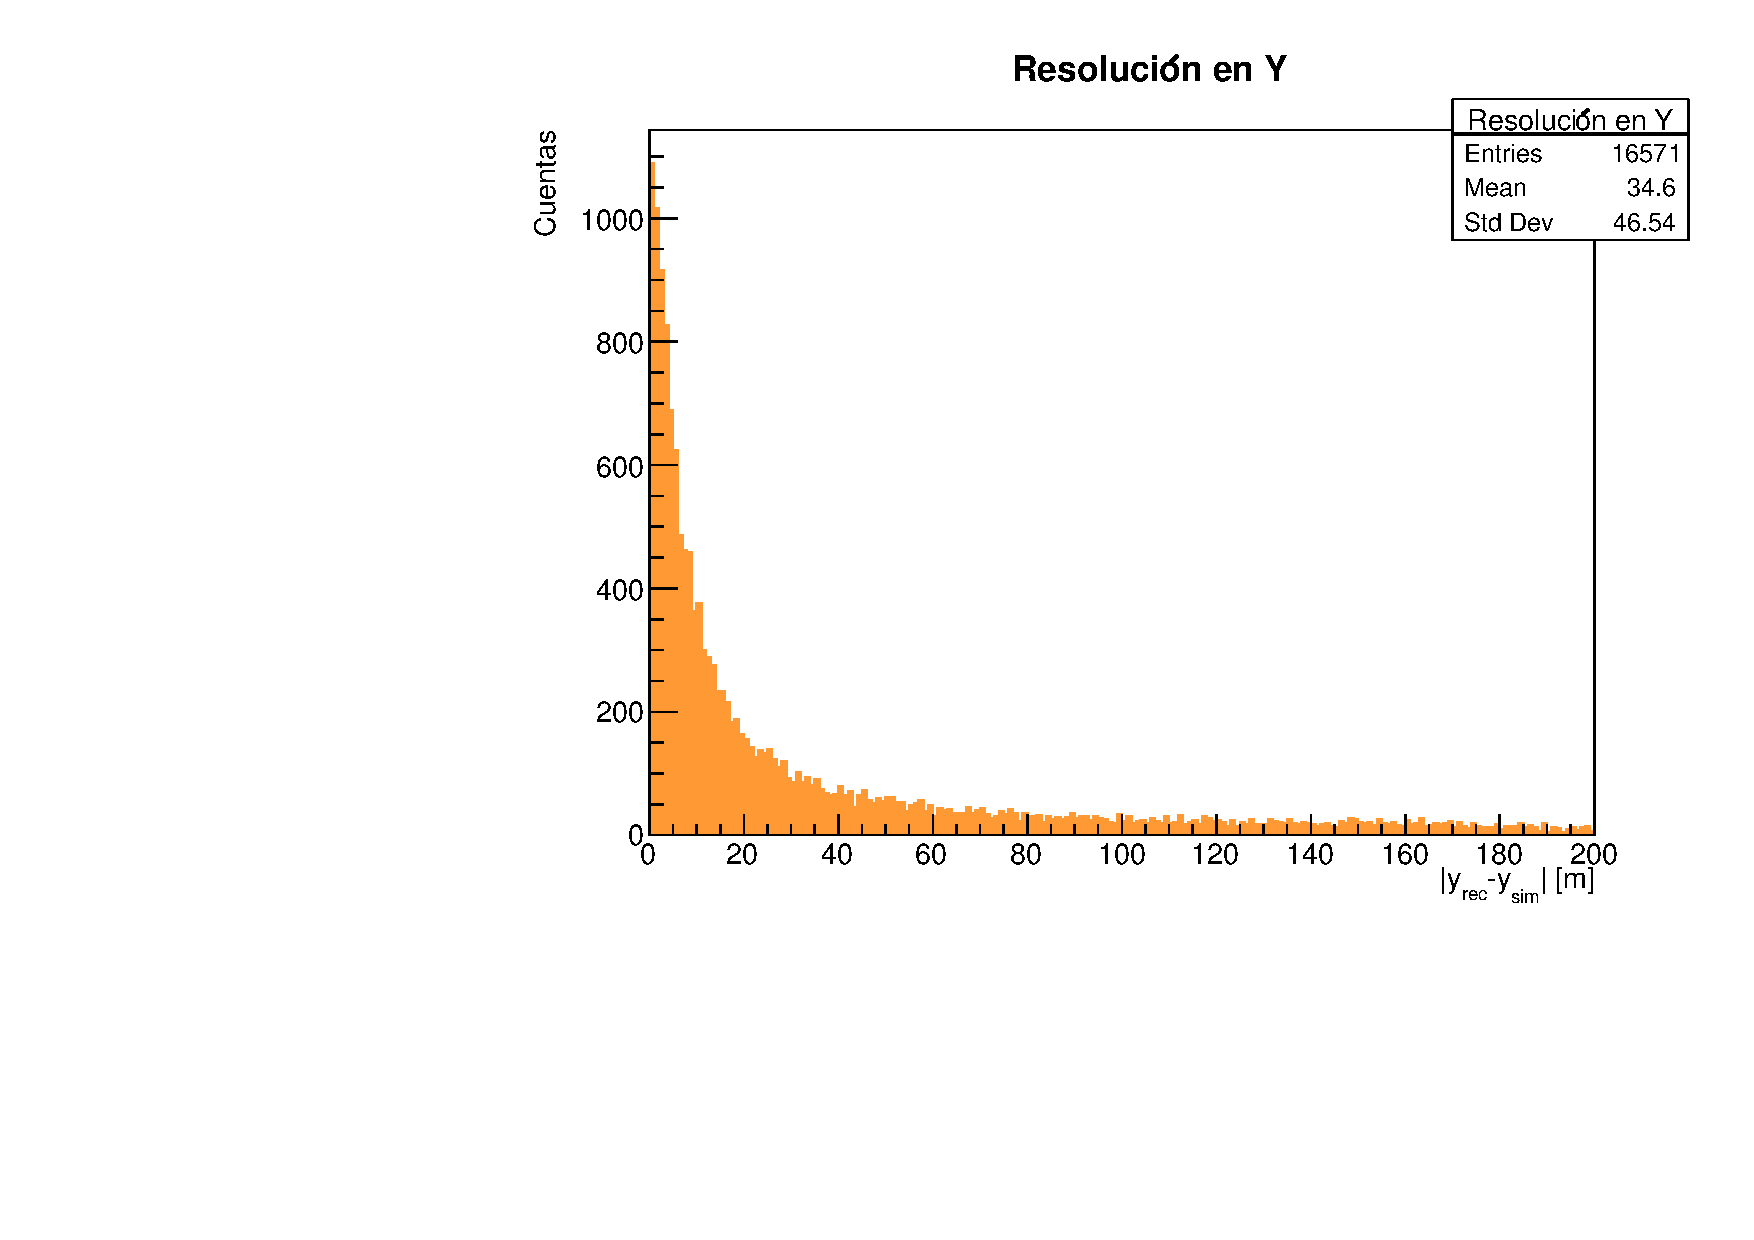
\includegraphics[width=0.8\textwidth]{../Figuras/Prob1B.pdf}}
\caption{Resolución en los ejes $X$, $Y$ tomando en cuenta todos los eventos.}
\label{fig:Prob1AB}
\end{figure}


\begin{figure}[H]
\centering
\subfloat[Resolución en el eje $X$, haciendo filtro con coreFiduScale]{
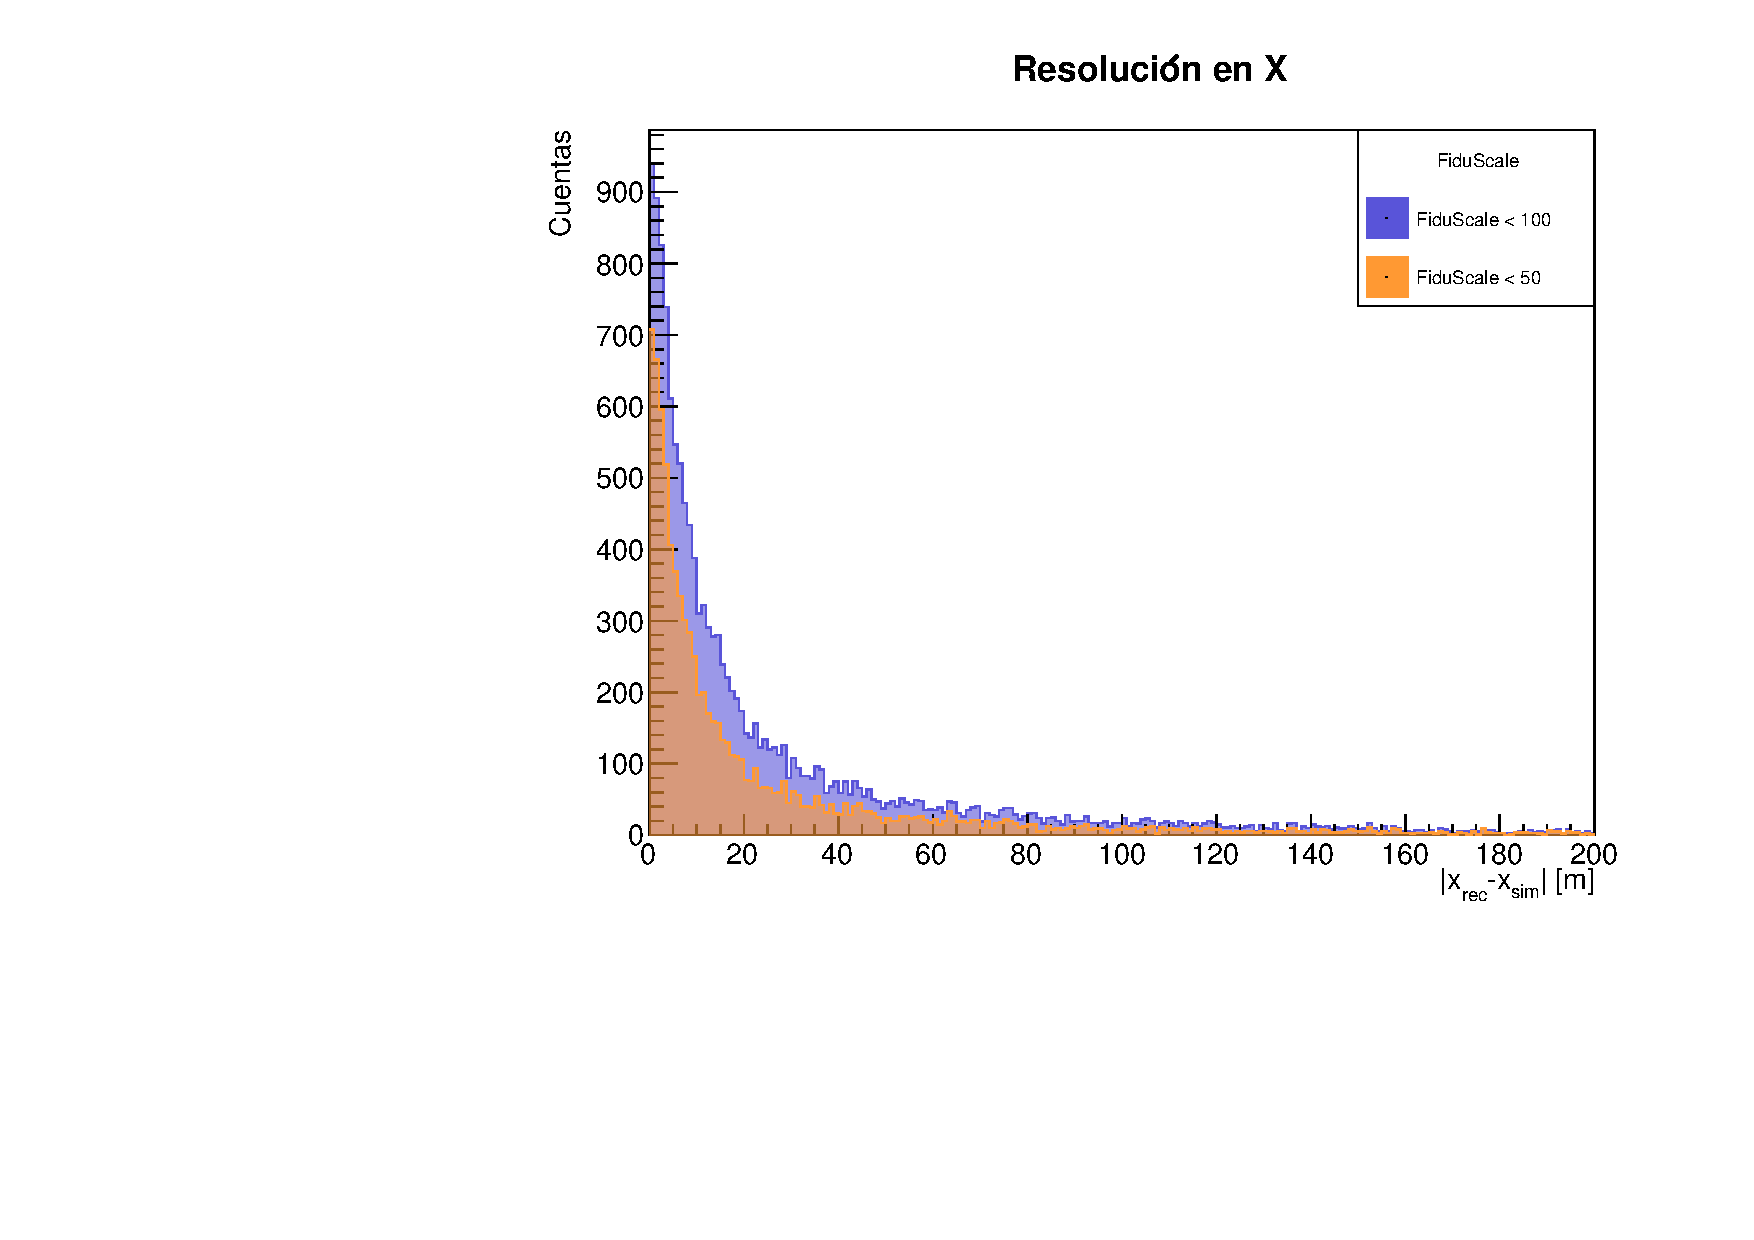
\includegraphics[width=0.8\textwidth]{../Figuras/Prob1C.pdf}}

\subfloat[Resolución en el eje $Y$, haciendo filtro con coreFiduScale]{
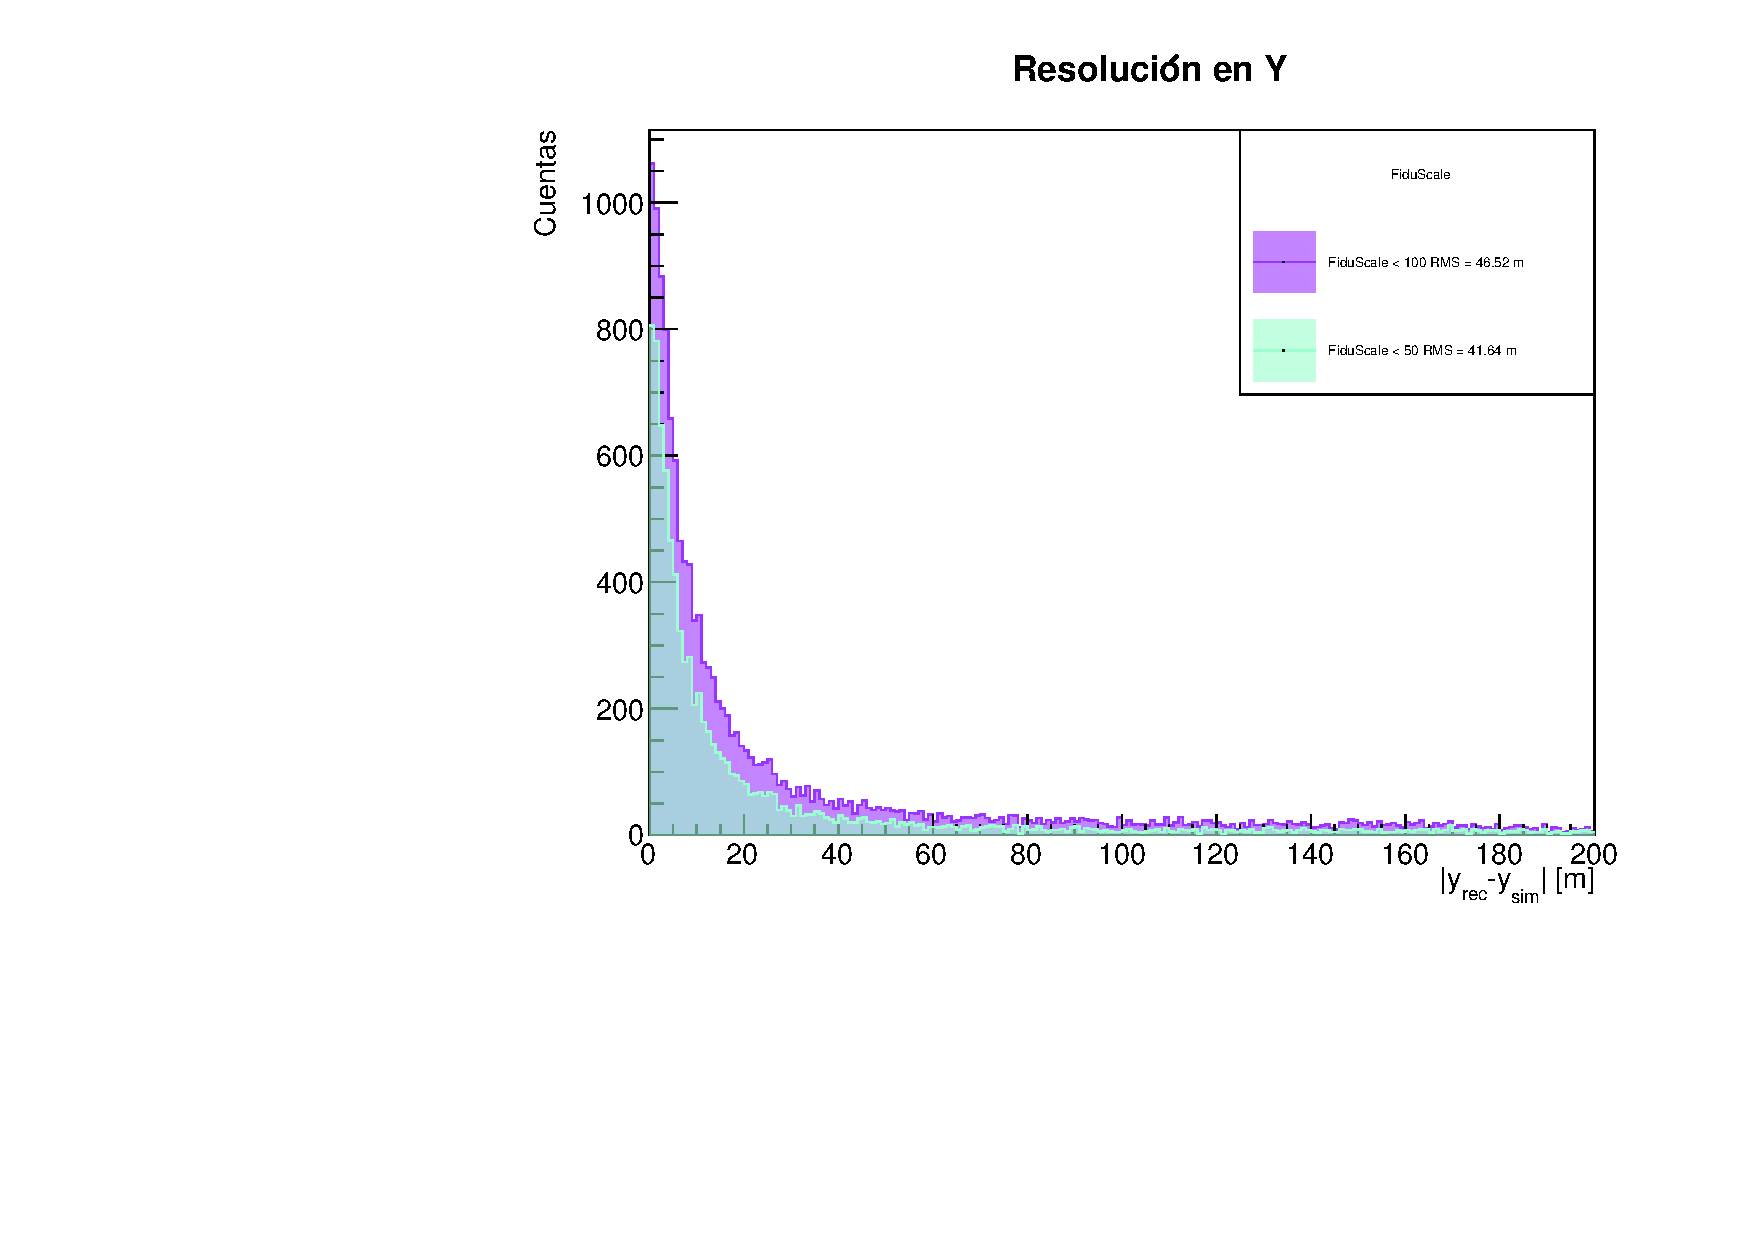
\includegraphics[width=0.8\textwidth]{../Figuras/Prob1D.pdf}}
\caption{Resolución en los ejes $X$, $Y$ haciendo un filtro con la variable coreFiduScale.}
\label{fig:Prob1CD}
\end{figure}

Al dividir los histogramas de acuerdo a la variable FiduScale no observamos alguna diferencia notable, más allá del hecho de que para FiduScale menor a 50 hay menos eventos. En todos los histogramas se aprecia que la mayor parte de los eventos cumplen que $|x_{\textrm	{rec}} -x_{\textrm{sim}}|=0$ y lo mismo con la dirección $y$. De las figuras \ref{fig:Prob1AB} se tiene que la resolución promedio en $x$ es $30$ m, mientras que en $y$ es 34.6 m.

\pagebreak
%%%%%%%%%%%%%%%%%%%%%%%%%%%%%%%%%%%%%%%%%%%%%%%%%%%%%%
\textbf{2)}
\begin{figure}[H]
\centering
\subfloat[Resolución del ángulo cenital para eventos con más y menos de 100 hits.]{
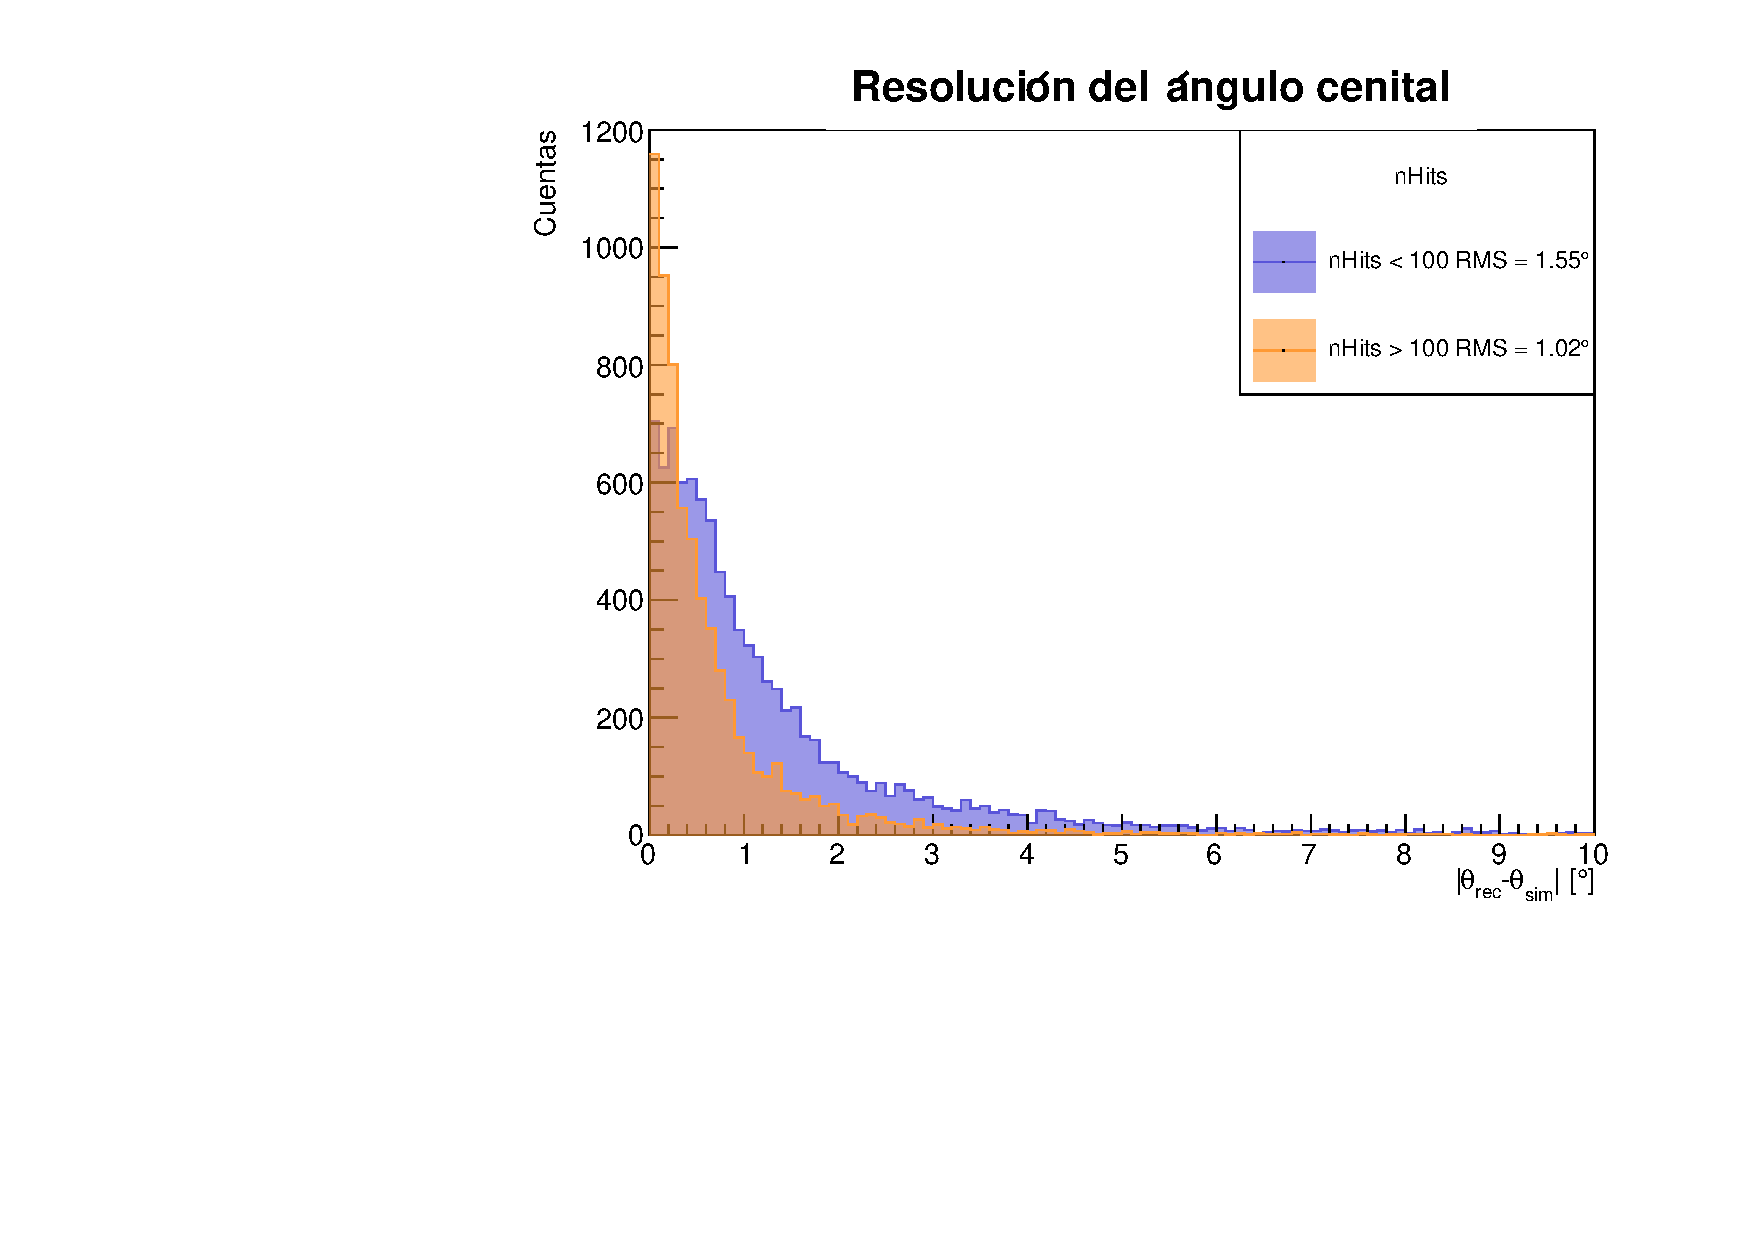
\includegraphics[width=0.78\textwidth]{../Figuras/Prob2A.pdf}}

\subfloat[Resolución del ángulo acimutal para eventos con más y menos de 100 hits.]{
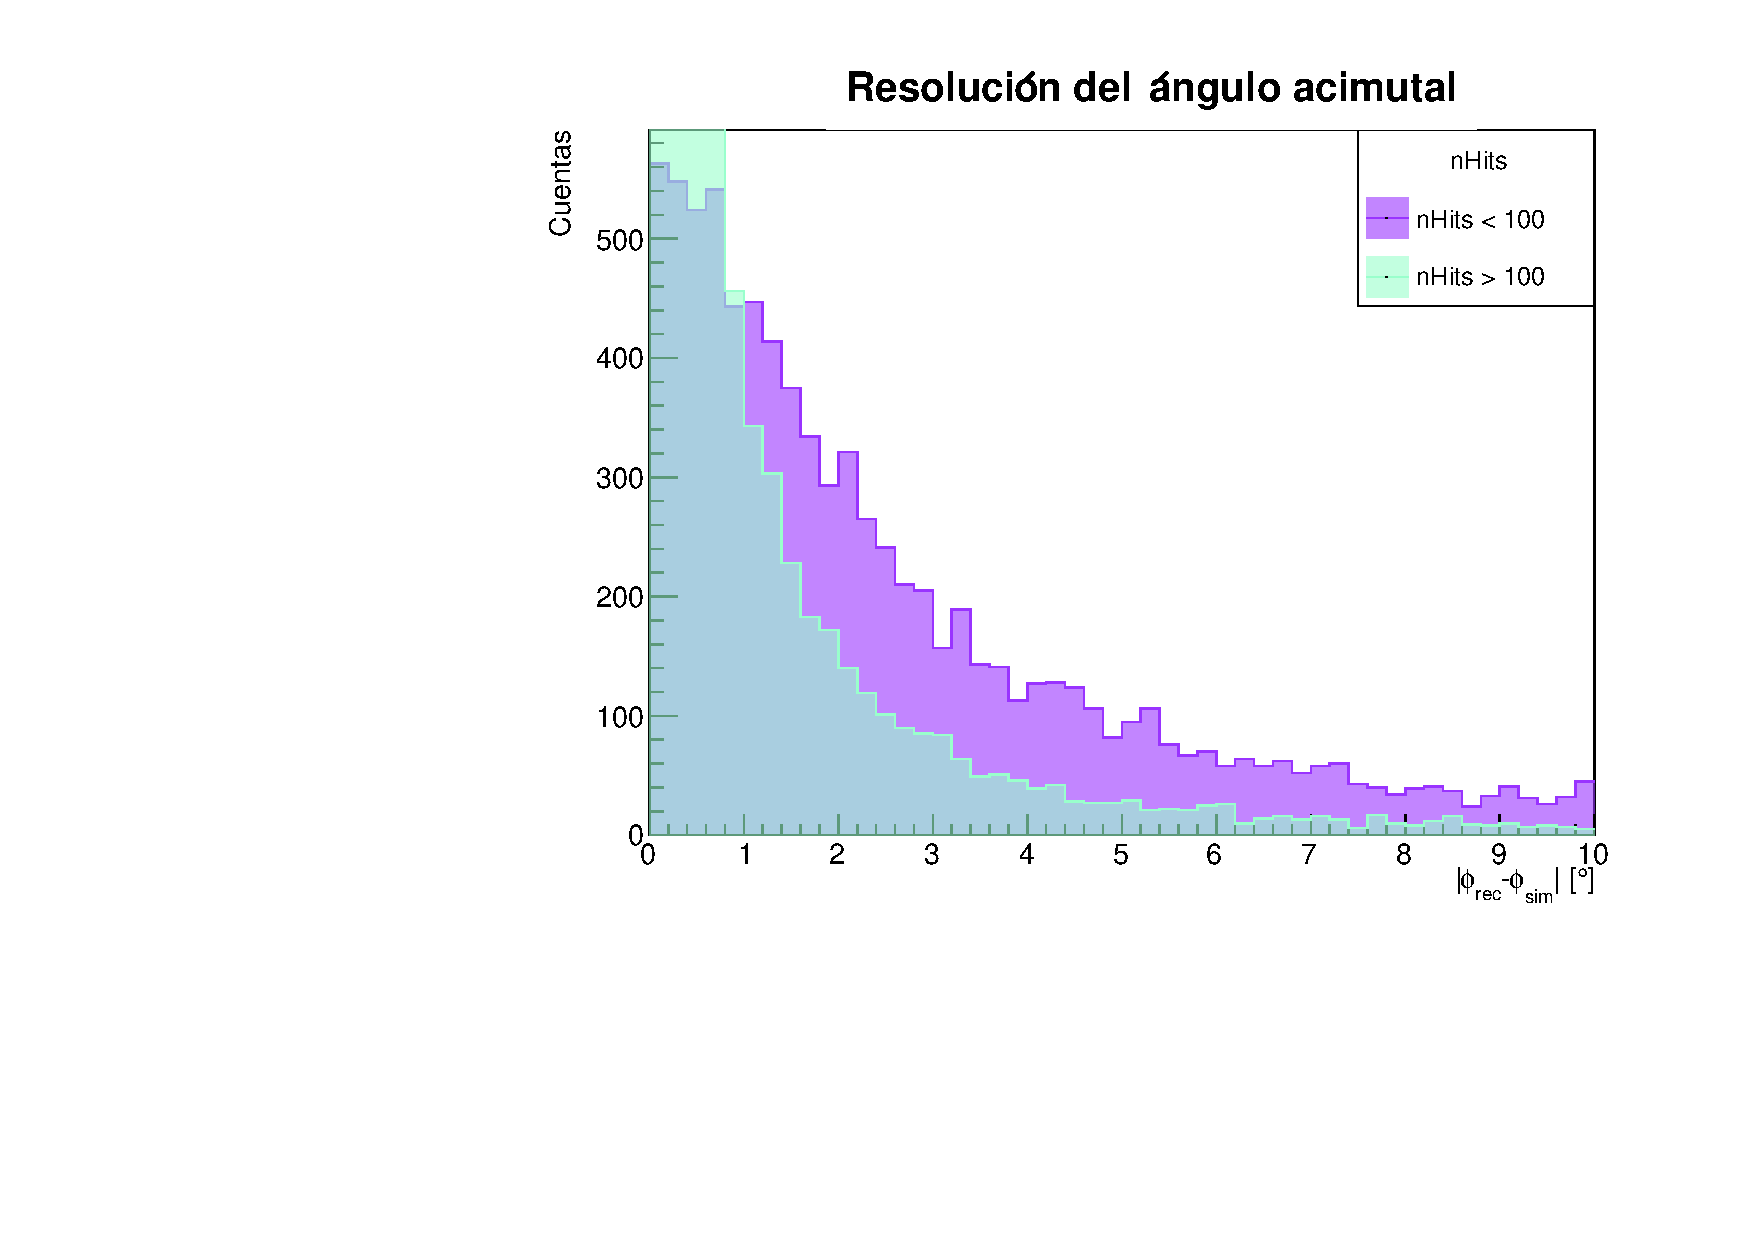
\includegraphics[width=0.78\textwidth]{../Figuras/Prob2C.pdf}}
\caption{Resolución de los ángulos cenital y acimutal tomando en cuenta el número de hits por evento.}
\label{fig:Prob2AC}
\end{figure}


\begin{figure}[H]
\centering
\subfloat[Resolución del ángulo cenital para eventos con diferente valor de coreFiduScale.]{
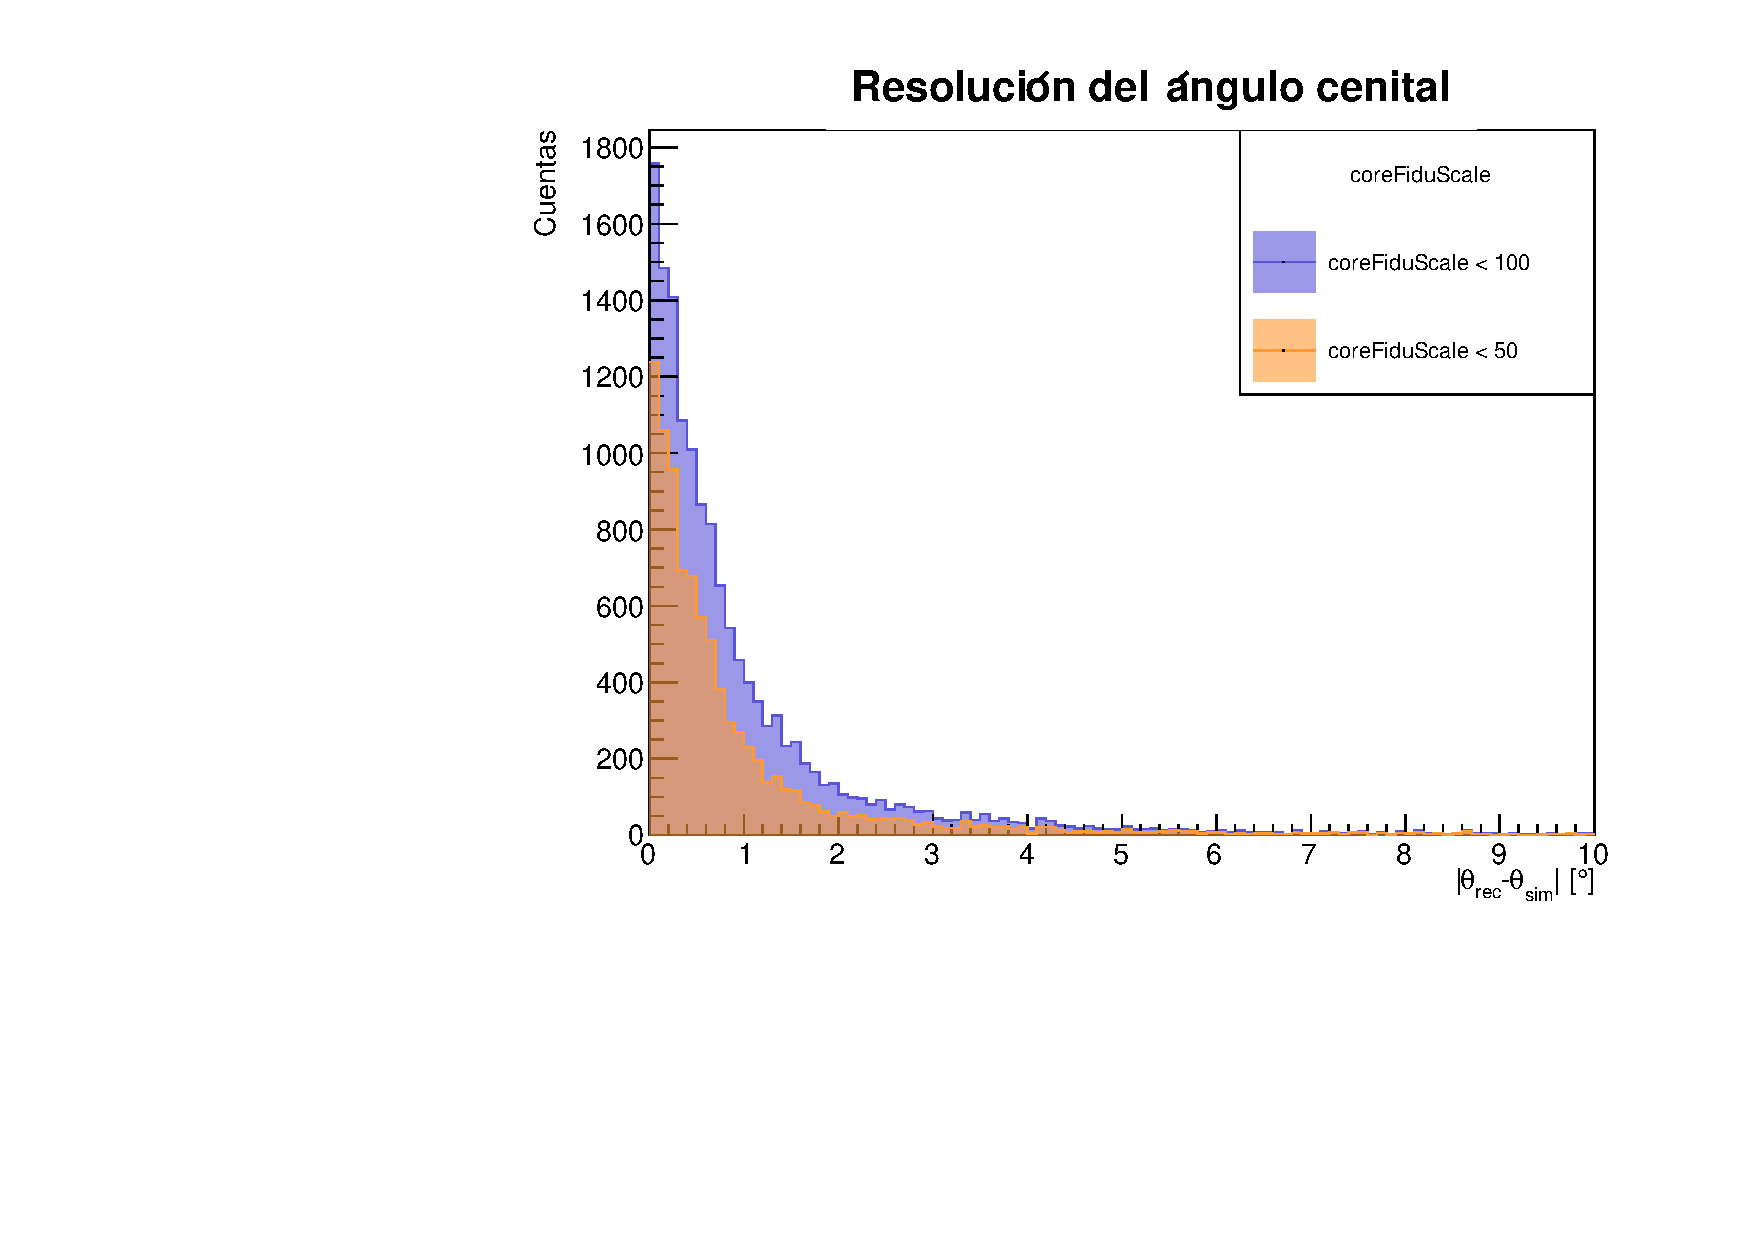
\includegraphics[width=0.78\textwidth]{../Figuras/Prob2B.pdf}}

\subfloat[Resolución del ángulo acimutal para eventos con diferente valor de coreFiduScale.]{
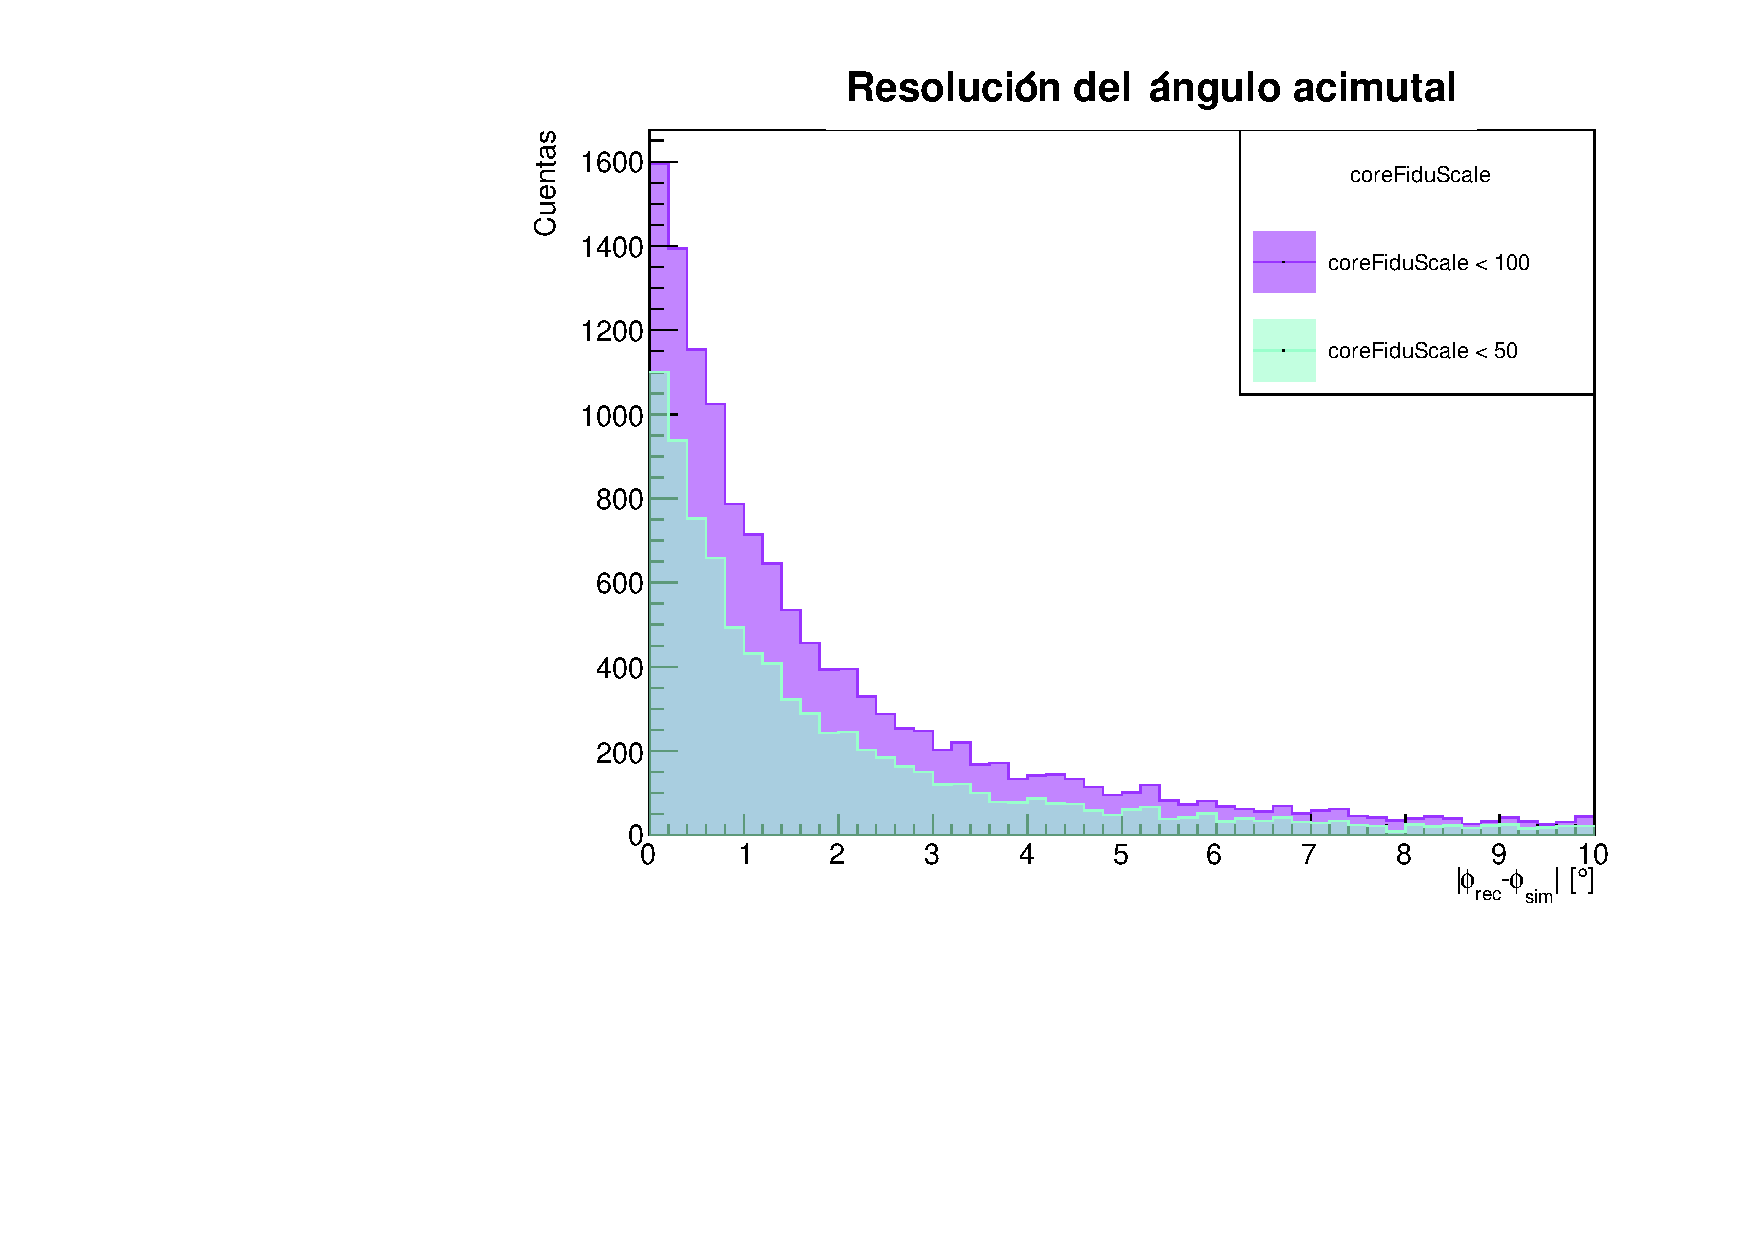
\includegraphics[width=0.78\textwidth]{../Figuras/Prob2D.pdf}}
\caption{Resolución de los ángulos cenital y acimutal tomando en cuenta la variable coreFiduScale.}
\label{fig:Prob2BD}
\end{figure}

Al hacer la comparación de acuerdo con el valor de la variable FiduScale, el comportamiento que se observa es el mismo que en el del problema anterior, en donde notamos que las distribuciones son bastante similares y sólo cambia el número de cuentas; incluso se observa que el valor RMS es muy similar. 

\hspace{5mm}Por otro lado, al dividir los eventos por número de hits, se observa que eventos con nHits$<100$ tienen menos cuentas cuyos valores de $|\theta_{\textrm	{rec}} -\theta_{\textrm{sim}}|$ o $|\phi_{\textrm	{rec}} -\phi_{\textrm{sim}}|$ sean cercanos a cero que para eventos con nHits$>100$. Sin embargo, para eventos con nHits$<100$ también sucede que hay más eventos cuyos valores de $|\theta_{\textrm	{rec}} -\theta_{\textrm{sim}}|$ o $|\phi_{\textrm	{rec}} -\phi{\textrm{sim}}|$ son superiores a 1° que en el caso de eventos con nHits$>100$. Además, el valor RMS cambia de forma más sustancial que al hacer la comparación con FiduScale. Esto sugiere que la resolución depende del número de hits.
\pagebreak

%%%%%%%%%%%%%%%%%%%%%%%%%%%%%%%%%%%%%%%%%%%%%%%%%%%%%%
\textbf{3)}
\begin{figure}[H]
\centering
\subfloat[Comparación entre la simulación y la reconstrucción a través de una red neuronal. Ajustamos una función lineal de la forma $y=a+bx$, los parámetros son $a=2.700(22)$, $b=0.209(6)$ (estos parámetros están en escala $\log_{10}$).]{
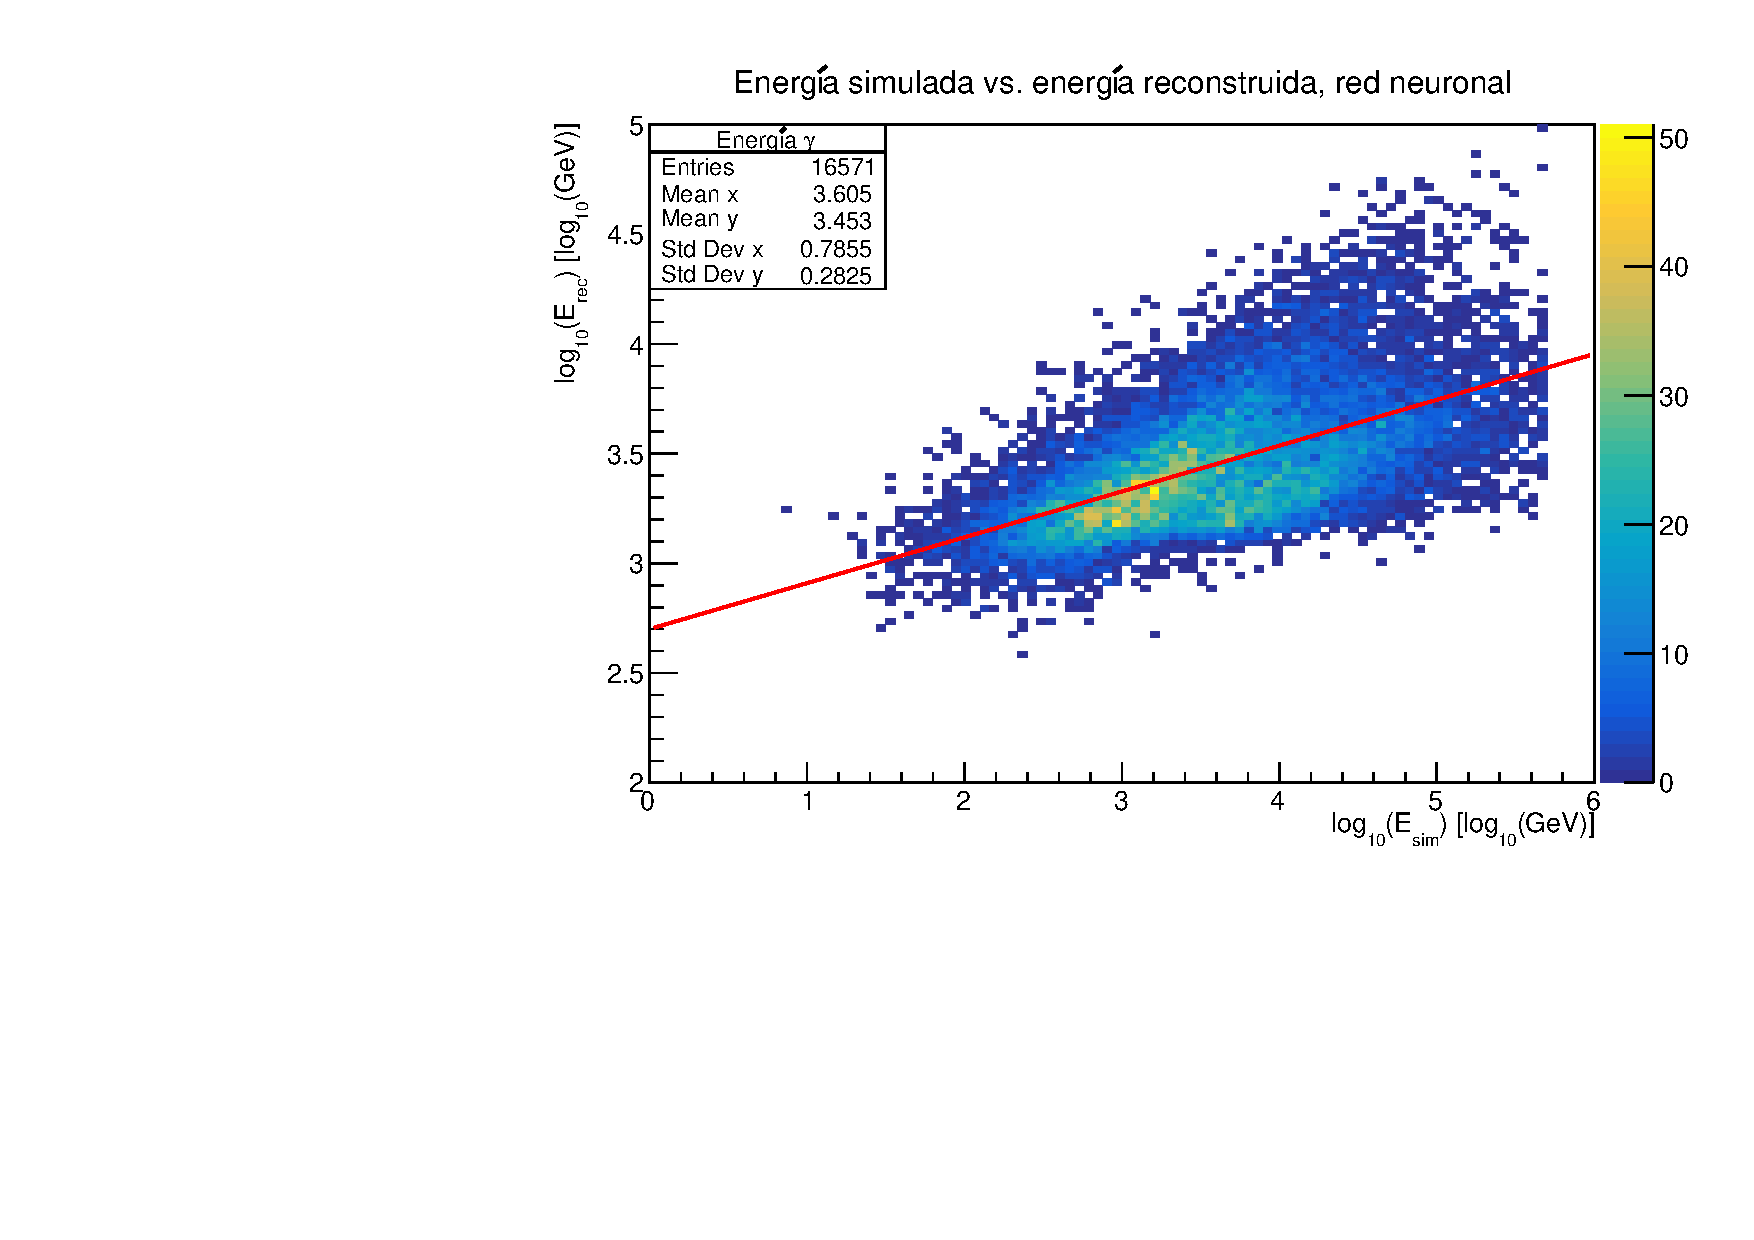
\includegraphics[width=0.7\textwidth]{../Figuras/Prob3A.pdf}}

\subfloat[Comparación entre la simulación y la reconstrucción a través del método ground parameter. Ajustamos una función lineal de la forma $y=a+bx$, los parámetros son $a=2.327(52)$, $b=0.236(14)$ (estos parámetros están en escala $\log_{10}$).]{
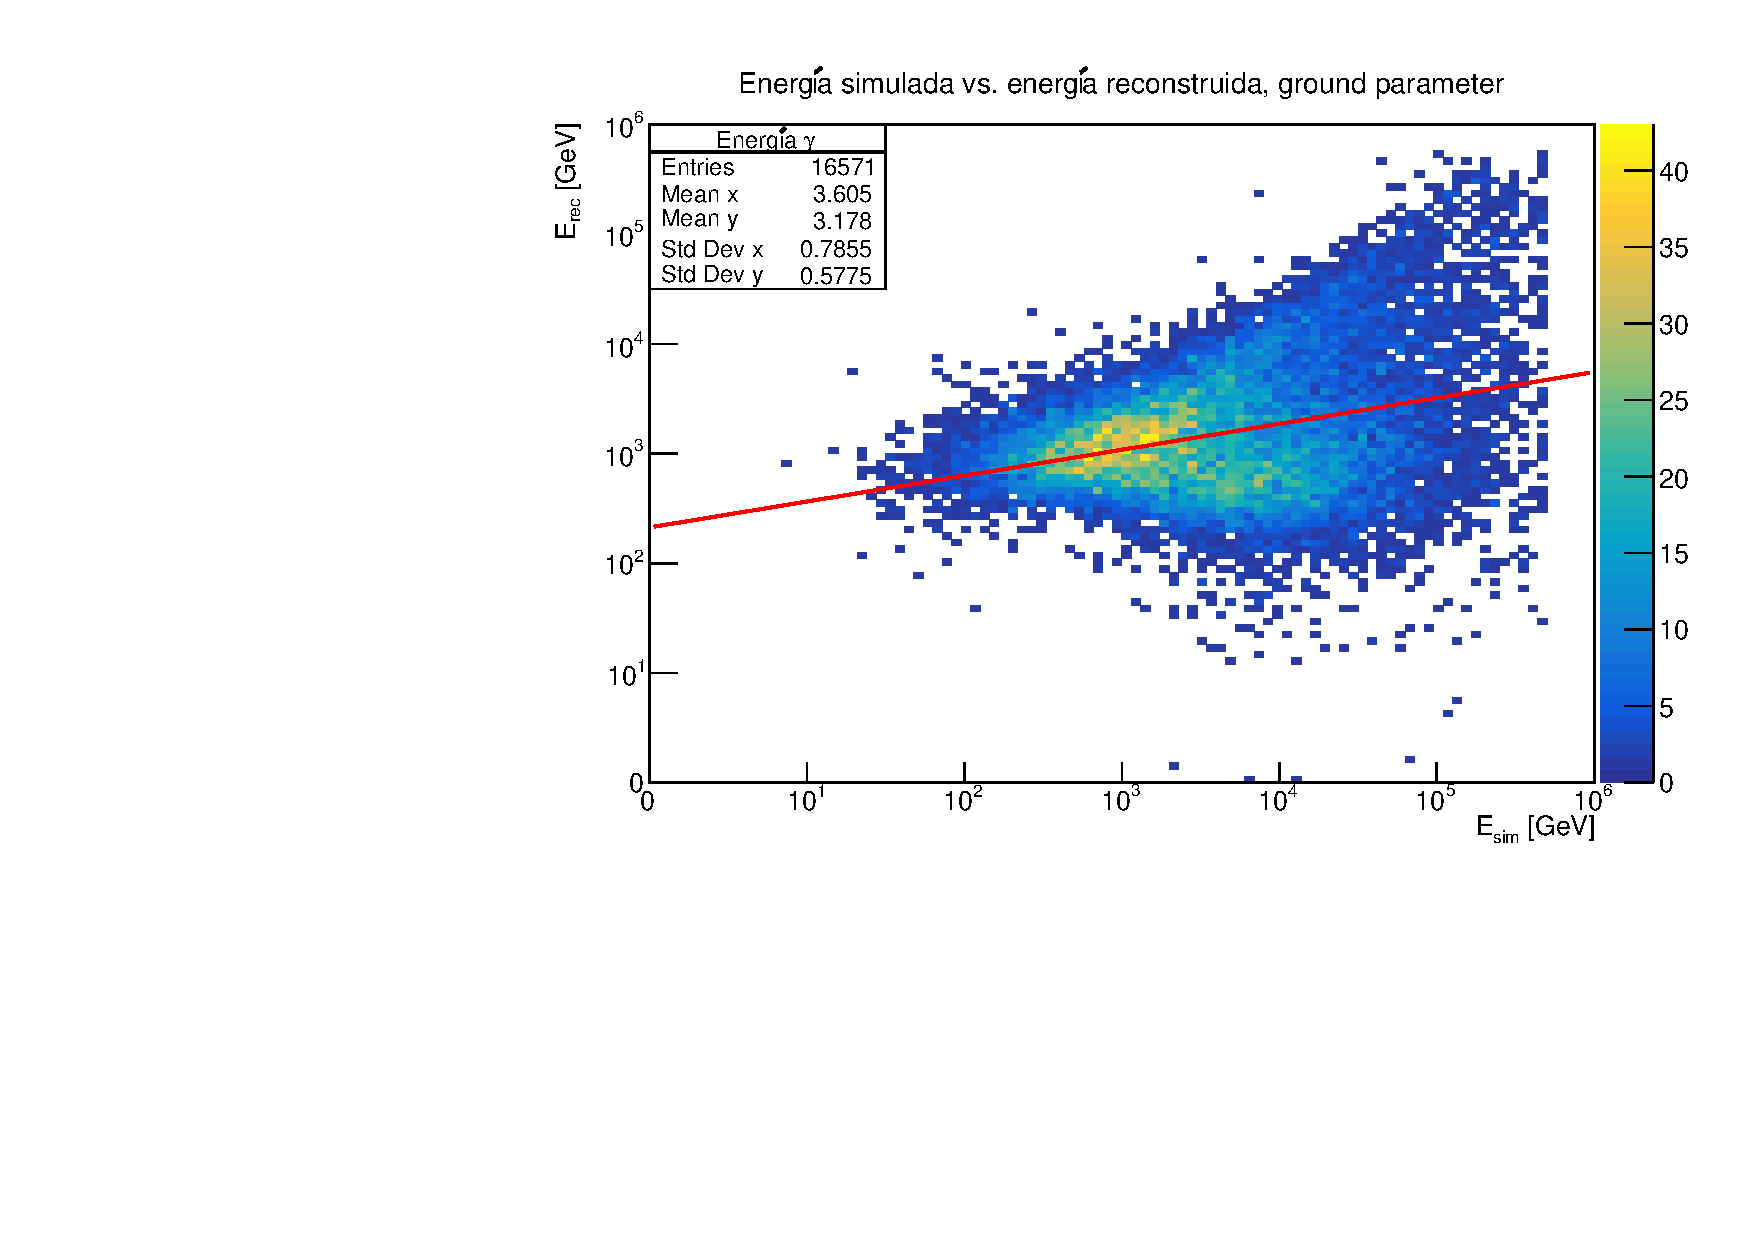
\includegraphics[width=0.7\textwidth]{../Figuras/Prob3B.pdf}}
\caption{Comparación entre la simulación y los diferentes algoritmos de reconstrucción de energía. La barra de colores indica el número de cuentas.}
\label{fig:Prob3}
\end{figure}

Se observa que para ground parameter la distribución está un poco más dispersa y reconstruye valores de energía que se encuentran por debajo de $10^2$ GeV, a diferencia de la red neuronal, que todos los valores de energía que reconstruye están por encima de $10^2$ GeV y en donde la distribución se encuentra menos dispersa. Así mismo, del ajuste lineal se observa que el valor de ambos parámetros $a$ y $b$ es bastante similar en ambos casos, no obstante en la red neuronal el error es más pequeño en dichos números. Con base todo lo anterior, concluimos que la red neuronal es mejor para reconstruir la energía.

\pagebreak
%%%%%%%%%%%%%%%%%%%%%%%%%%%%%%%%%%%%%%%%%%%%%%%%%%%%%%

\textbf{4)}
\begin{figure}[H]
\centering
\subfloat[Distribución de energía para eventos con energías entre 1 y 5 TeV para $\theta<20^\circ$]{
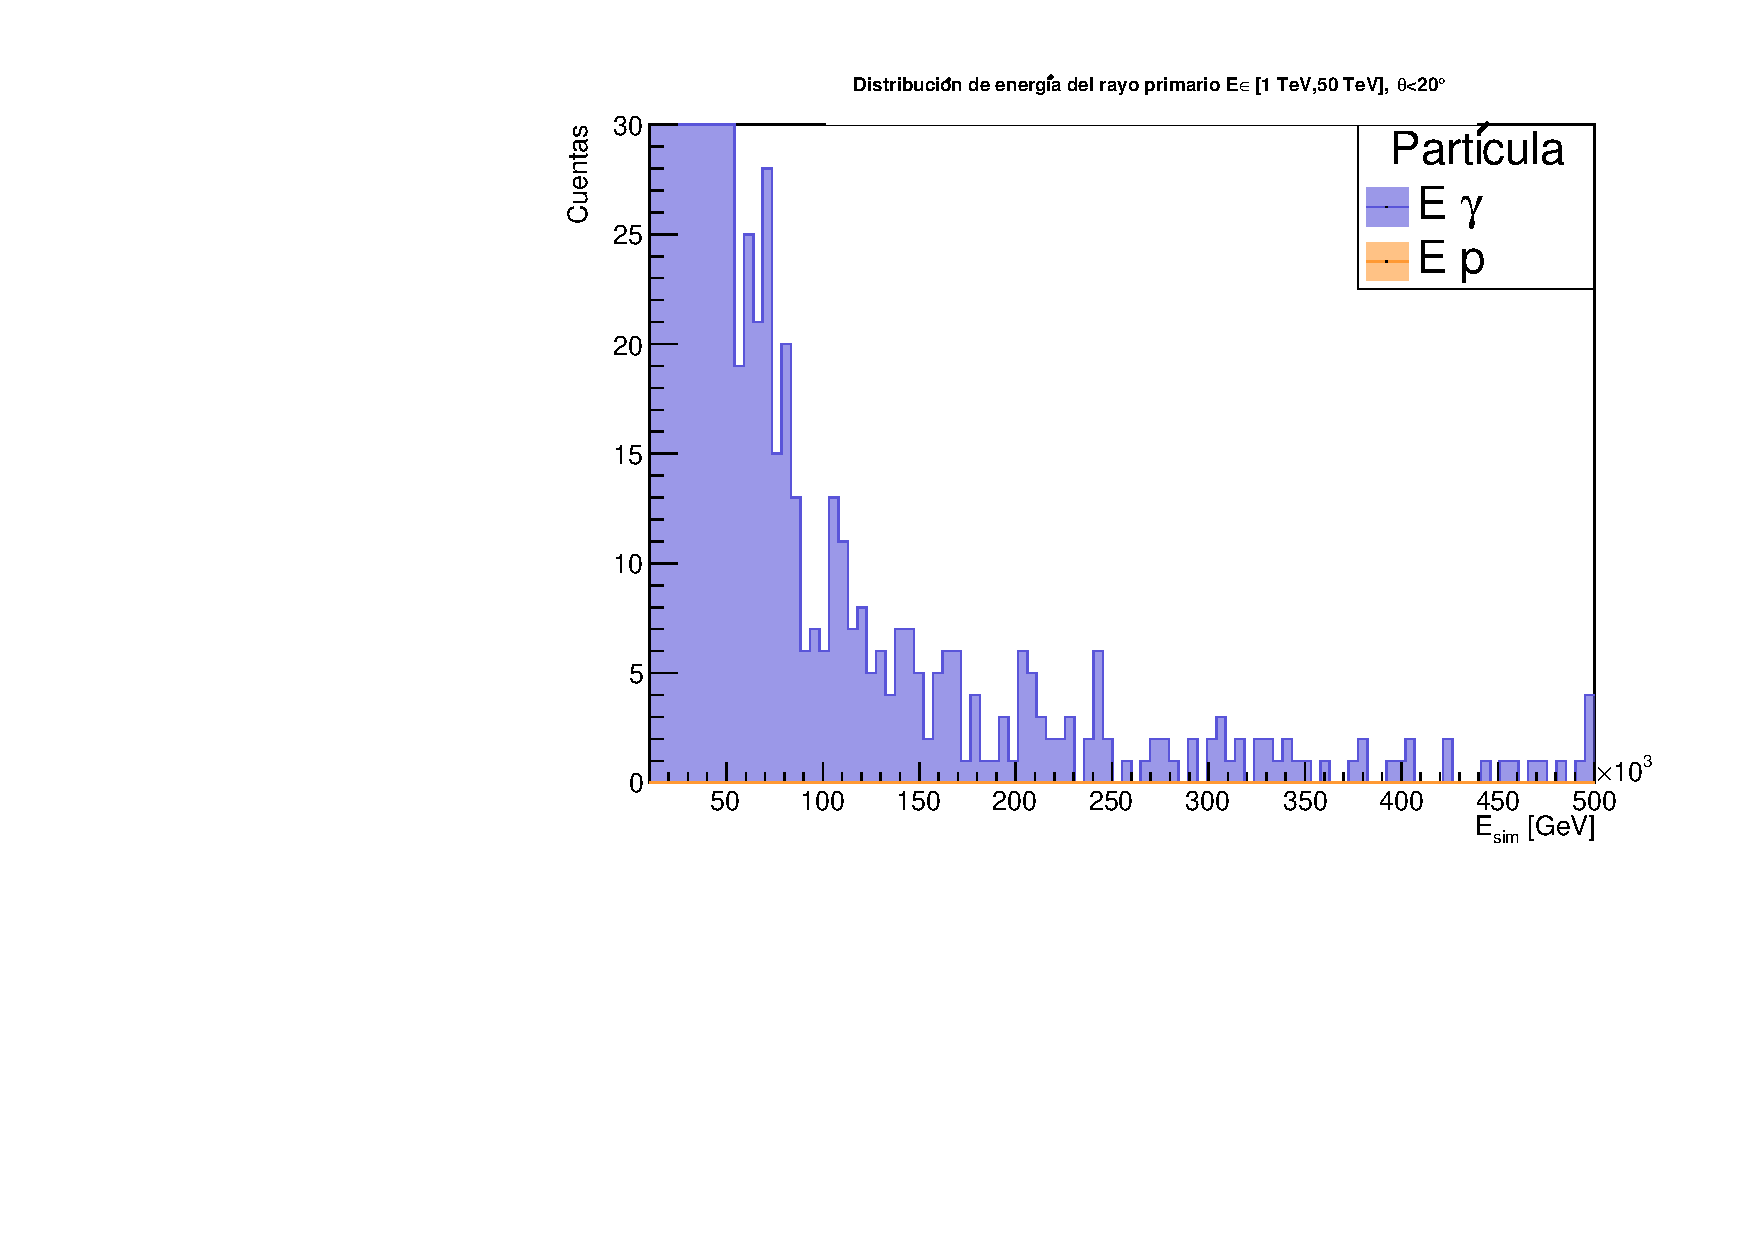
\includegraphics[width=0.78\textwidth]{../Figuras/Prob4A.pdf}}

\subfloat[Distribución angular $\theta$ para ambos tipos de partículas. Consideramos todo los eventos.]{
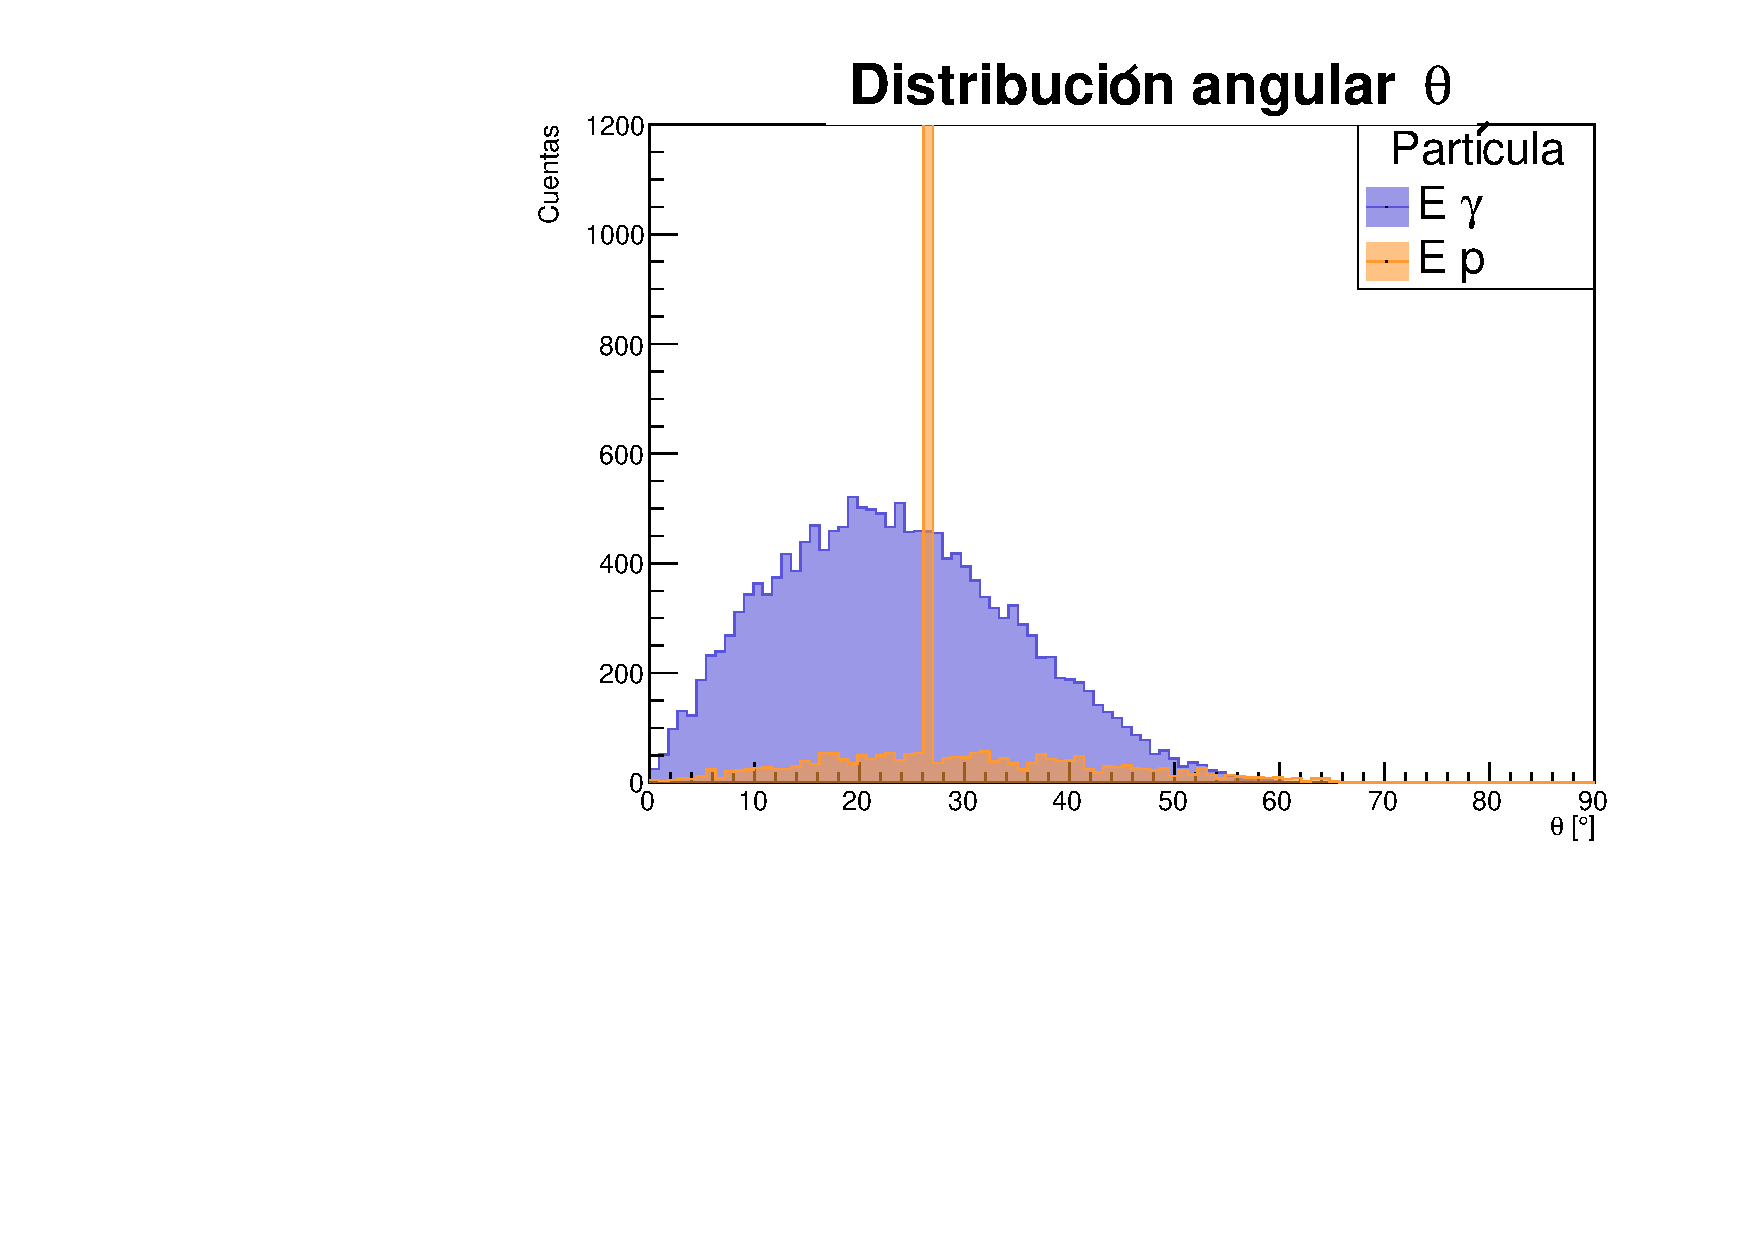
\includegraphics[width=0.78\textwidth]{../Figuras/Prob4B.pdf}}
\end{figure}
\begin{figure}[H]
\centering
\subfloat[Distribución angular $phi$ para ambos tipos de partículas. Consideramos todos los eventos.]{
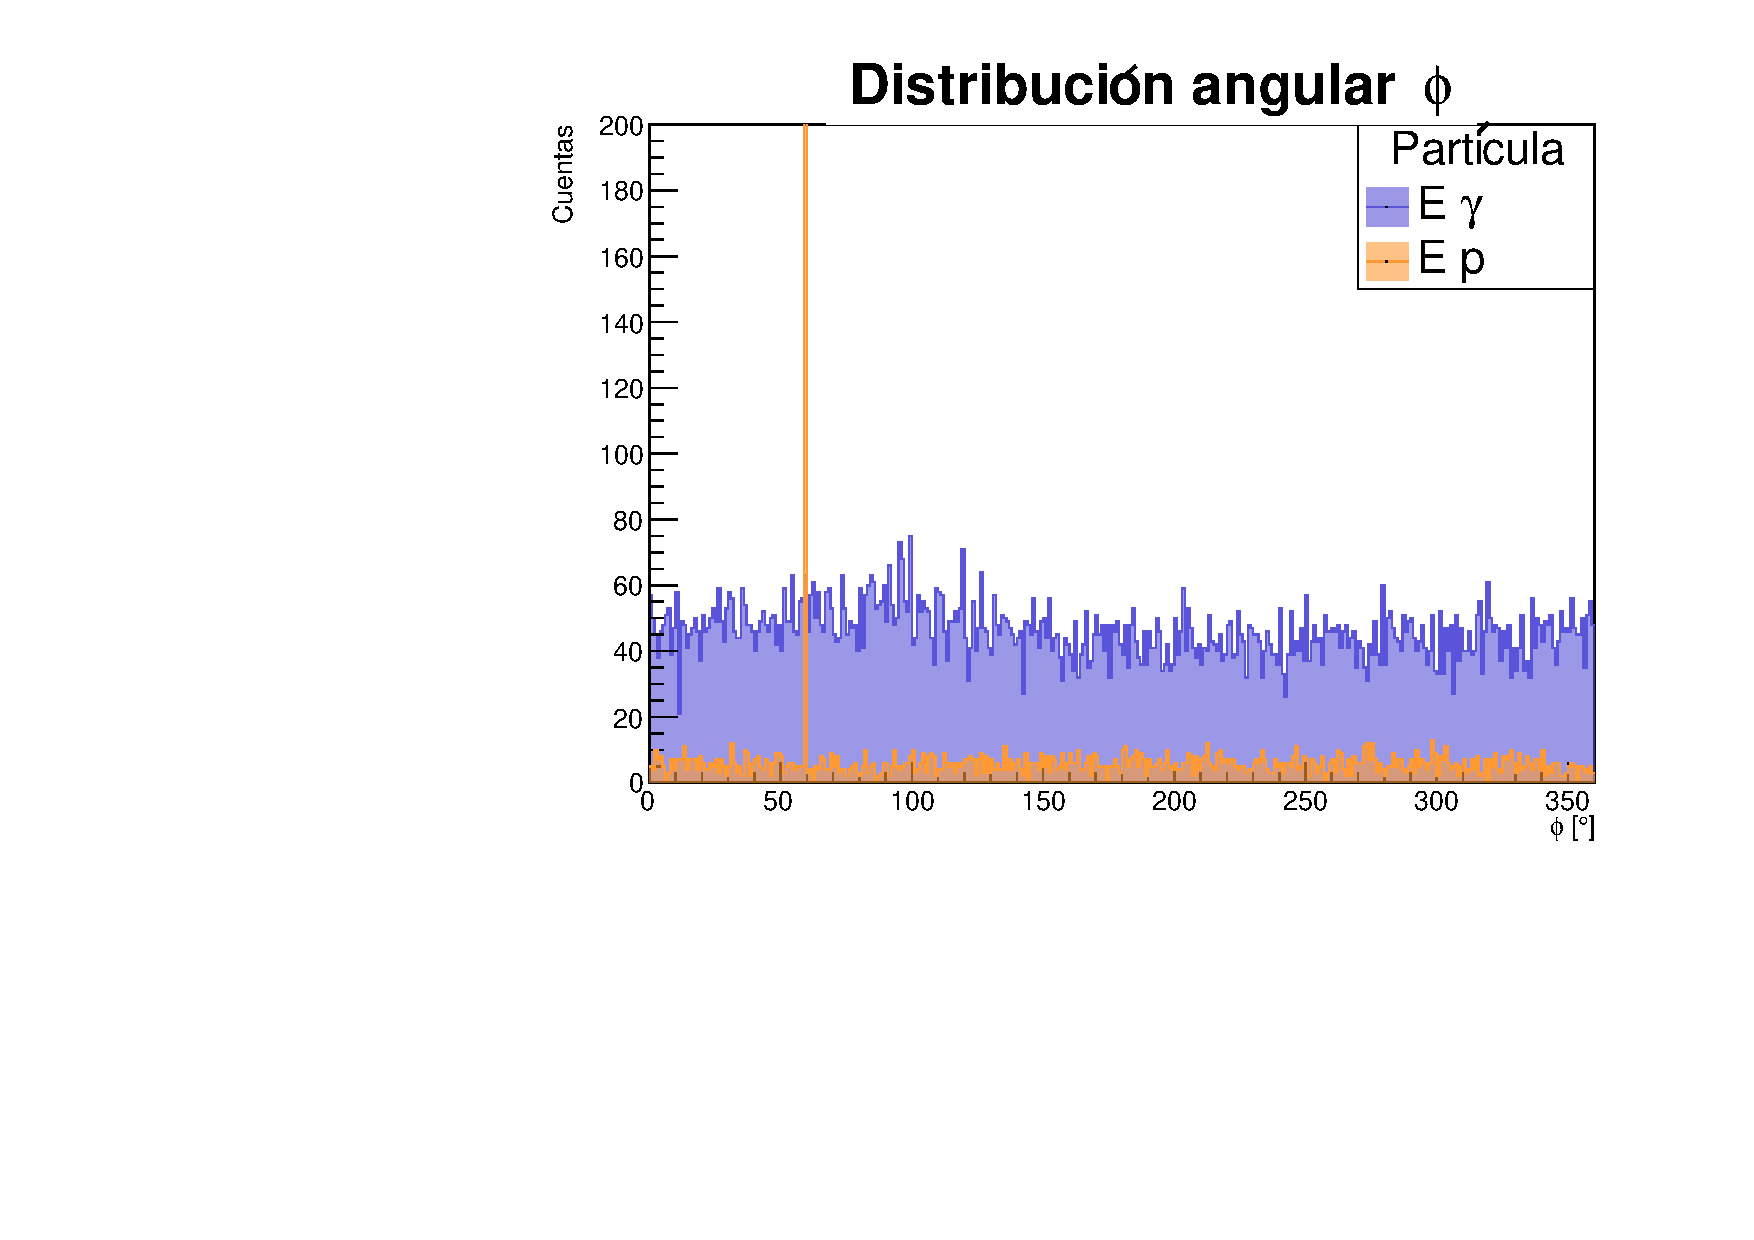
\includegraphics[width=0.78\textwidth]{../Figuras/Prob4C.pdf}}
\caption{Histogramas de energía y distribuciones angulares de los dos tipos de partículas primarias.}
\label{fig:Prob4}
\end{figure}
Al comparar las distribuciones de energía para $E\in[1, 5]$ TeV y $\theta<20^{\circ}$, figura \ref{fig:Prob4} (a), se observa que prácticamente no hay eventos registrados para los protones en esos rangos. Esto podría indicar una diferencia entre la forma de detectar entre ambas partículas, sin embargo no es totalmente concluyente ya que el archivo de datos de protones contiene muchos menos eventos que el de fotones. 

\hspace{5mm}Por otro lado, en la distribución angular $\theta$, figura \ref{fig:Prob4} (b), observamos que los protones tienen un pico muy marcado, que posiblemente sea algún fallo con la simulación; además, un pico similar se encuentra en la distribución de $\phi$. No obstante, si ignoramos el pico de la distribución angular $\theta$, podemos darnos cuenta de que aún así el máximo de la distribución para $\gamma$'s y $p$'s no es lo mismo, lo cual nos lleva a considerar que la distribución angular de estas partículas puede ser diferente debido a que no tienen la misma carga y sabemos que el campo magnético de la Tierra afecta la trayectoria de las partículas. De la distribución $\phi$ no se puede concluir nada. 
\end{document}